\chapter{The Variable Library}
\label{chap:variable-library}

\emph{Variables} in Opus and UrbanSim represent quantities of interest.
These variables can be used in two principal ways: in specifying models and
in computing indicators to assess simulation results.  For example, a
\mbox{\tt distance\_to\_highway} variable might be used to help predict land
values or or household location choices; and a \mbox{\tt population\_density}
variable might be used in computing indicators that are useful for
evaluating simulation results.  The variable library is a repository for
variables defined in the system that are accessible from the GUI\@.  Since
it provides a resource that is used throughout the GUI, we access it from
the tools menu on the menu bar at the top of the main window, as in Figure
\ref{fig:variable-library-menu}.  The screenshot in Figure
\ref{fig:variable-library-popup} shows a popup window that appears once a
user selects the variable library option on the tools menu.  Note that the
contents of it depend on what project is loaded.  In this case, we have the
eugene\_parcel project loaded, and see the variables that are initially
available in this project.

Datasets and variables are explained in considerably more detail in
Chapters \ref{chap:data-in-opus} and \ref{chap:creating-variables}.
Briefly for now, there are three ways to define a variable:

\begin{itemize}

\item A variable can be defined using an expression written in a
  domain-specific programming language.  There is a brief description of
  the language later in this chapter, and a more complete description in
  Section \ref{sec:expressions}.  We'll be concentrating on this option in
  this chapter.

\item A variable can also be a primary attribute of a dataset (think of
  these as columns in the input database).

\item Finally, a variable can be defined as a Python class.  This is an
  advanced option for complicated variables beyond the scope of the
  domain-specific programming language --- we'll use variables defined this
  way, but for now won't write any new ones.

\end{itemize}

\begin{figure}[htp]
\begin{center}
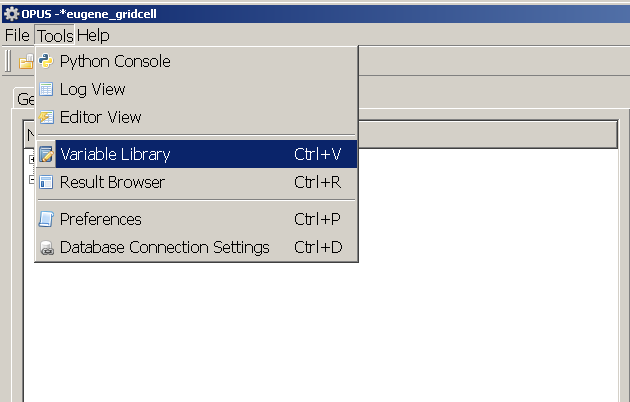
\includegraphics[scale=0.6]{part-gui/images/model-manager-variable-library-menu.png}
\end{center}
\caption{Opening the Variable Library from the ``Tools'' Menu}
\label{fig:variable-library-menu}
\end{figure}

\begin{figure}[htp]
\begin{center}
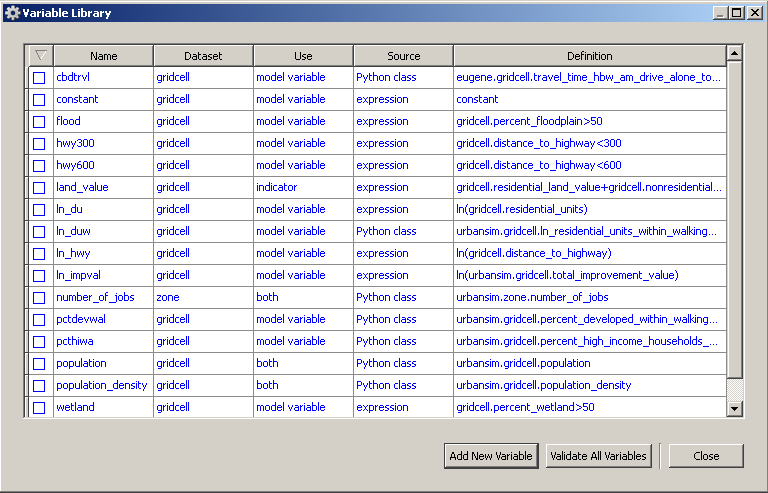
\includegraphics[scale=0.6]{part-gui/images/model-manager-variable-library-popup.png}
\end{center}
\caption{Variable Library Popup Window}
\label{fig:variable-library-popup}
\end{figure}

Note the buttons at the bottom of this window to add new variables or
validate all variables.  Adding a new variable defined as an expression is
straightforward.  There are examples of existing variables defined using
expressions in the variable library window --- look for variables with the
entry ``expression'' in the ``Source'' column.  The corresponding variable
definition is in the right-most column.  Note that this definition is
executable code --- it's not just a description.  Expressions are built up
as functions and operations applied to existing variables in the library.
For example, the expression for wetland is defined as
\mbox{\tt gridcell.percent_wetland>50}.  This defines the creation of a
true/false, or boolean, variable that is interpreted as 1 if the gridcell
has more than 50 percent coverage by wetland, 0 otherwise.  Variables are
array-valued, so we are actually computing an array of true/false values
for every gridcell with the single expression.

If you click on the add new variable button at the bottom of the variable
library window, it opens a dialog box as shown in Figure
\ref{fig:variable-library-new-variable}.  The top entry is the name you
want to use for the variable.  Let's say we want to create a new variable
that is a log of population density.  We already have a population density
variable defined by gridcell, so we can just take the log of this value.
Let's name the variable ln\_population\_density, leave the middle selection
as ``expression,'' and fill in a simple expression in the definition
area: \mbox{\tt ln(gridcell.population_density)}.  Note that the dialog box
provides two buttons to help you check your new variable.  The check syntax
button tests whether the expression you have entered passes the Python and
expression syntax checkers -- in other words, is it syntactically correct.
The second allows you to test whether if you apply this expression to your
available data, it can successfully compute a result.  This is very helpful
in determining whether you might have referred to a data element that is
not present, or is otherwise not computable with your data.  In short,
these two tools allow testing whether the variables are in a state that can
be computed on the available data.

\begin{figure}[htp]
\begin{center}
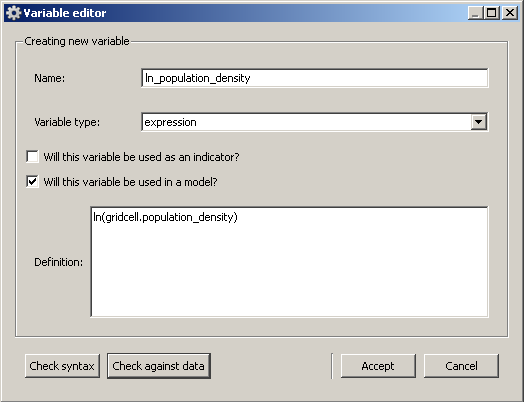
\includegraphics[scale=0.6]{part-gui/images/model-manager-variable-library-new-variable.png}
\end{center}
\caption{Adding a New Variable}
\label{fig:variable-library-new-variable}
\end{figure}

We just saw an example of using an expression to define the 
\mbox {\tt ln\_population\_density} variable.  More generally, a new
variable can be defined in terms of existing variables, where these
existing variables are referenced as a ``qualified name'' consisting of the
dataset name and the variable name, for example, 
\mbox{\tt gridcell.population\_density}.  Or our new variable can be used
in yet another definition by writing \emph{its} qualified name: 
\mbox{\tt gridcell.ln\_population\_density}.

In building up an expression, we can apply various functions to other
variables or subexpressions.  The available functions include {\tt ln},
{\tt exp}, and {\tt sqrt}.  Also, we can use the operators from the numpy
package, including {\tt + - * / **} (where {\tt **} is exponentiation).
Again, the expressions are all array-valued, so that 
\mbox{\tt ln(2*gridcell.population\_density)} is an array, 
consisting of the logs of 2 times the population density of each grid cell.
